\chapter{SOLID}

\section{Analyse Single-Responsibility-Principle (SRP)}

\subsubsection{Positiv-Beispiel:}

\begin{wrapfigure}{r}{0.40\textwidth}
	\centering
	\vspace{-30pt} % Manchmal möchte man den oberen Abstand selbst anpassen
	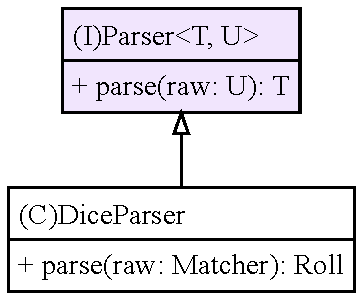
\includegraphics[width=0.30\textwidth]{Bilder/DiceParser_structure.pdf}
	\vspace{-10pt}
	% Das folgende ist ein Trick, um "Abbilgung x.y" in eine
	% eigene Zeile zu packen. Der Text zwischen [ und ] steht
	% im Abbildungsverzeichnis. Der Text darunter wird
	% tatsächlich angezeigt.
	\caption[UML-Diagramm von ase.plugin.cli.parsers.DiceParser.]{\unskip}
	UML-Diagramm von \textit{ase.plugin.cli.parsers.DiceParser}.
	\label{fig:srp-DiceParser}
\end{wrapfigure}

\autoref{fig:srp-DiceParser} zeigt das UML-Klassendiagramm des \textit{DiceParser}, welcher in der Plugin-Schicht
unter \texttt{plugin.cli.parsers} zu finden ist und das Positivbeispiel darstellt. 
Dieser implementiert das \textit{Parser}-Interface aus 
\texttt{plugin.cli}. Die einzige Aufgabe des DiceParsers ist es die Usereingabe zum Erstellen eines Würfelwurfs
aus Text zu parsen und das entsprechende Objekt zu kreieren. Hierzu wird der \textit{Regex}-Matcher, der 
bereits den Syntax überprüft hat an die \textit{parse}-Methode übergeben und daraus die Arugmente extrahiert, 
um den \textit{Roll} zu erstellen.

\subsubsection{Negativ-Beispiel:}

\autoref{fig:srp-RollHandler} zeig das UML-Klassendiagramm des \textit{RollHandler}, welcher in der Applikations-Schicht
die Würfelwürfe für die Rettungen (\textit{Endeavor}) \underline{und} Kämpfe (\textit{Encounter}) bearbeitet. 
Hierbei entscheidet die öffentliche \textit{handle}-Methode, ob es sich um einen Encounter oder ein Endeavor handelt
(dies ist allerdings eigentlich schon bei Aufruf dieser bekannt)
und führt die entsprechende private Methode aus. Die Klasse hat also zwei Aufgaben (Responsibilities). \\
Um dies zu lösen kann einfach die Klasse \textit{RollHandler} in zwei Klassen aufgeteilt werden - 
den \textit{EncounterHandler} und \textit{EndeavorHandler} - die nun jeweils nur noch genau eine Aufgabe haben 
und somit das SRP einhalten, wie \autoref{fig:srp-RollHandler-fixed} zeigt. 

\begin{figure}[H]
	\centering
	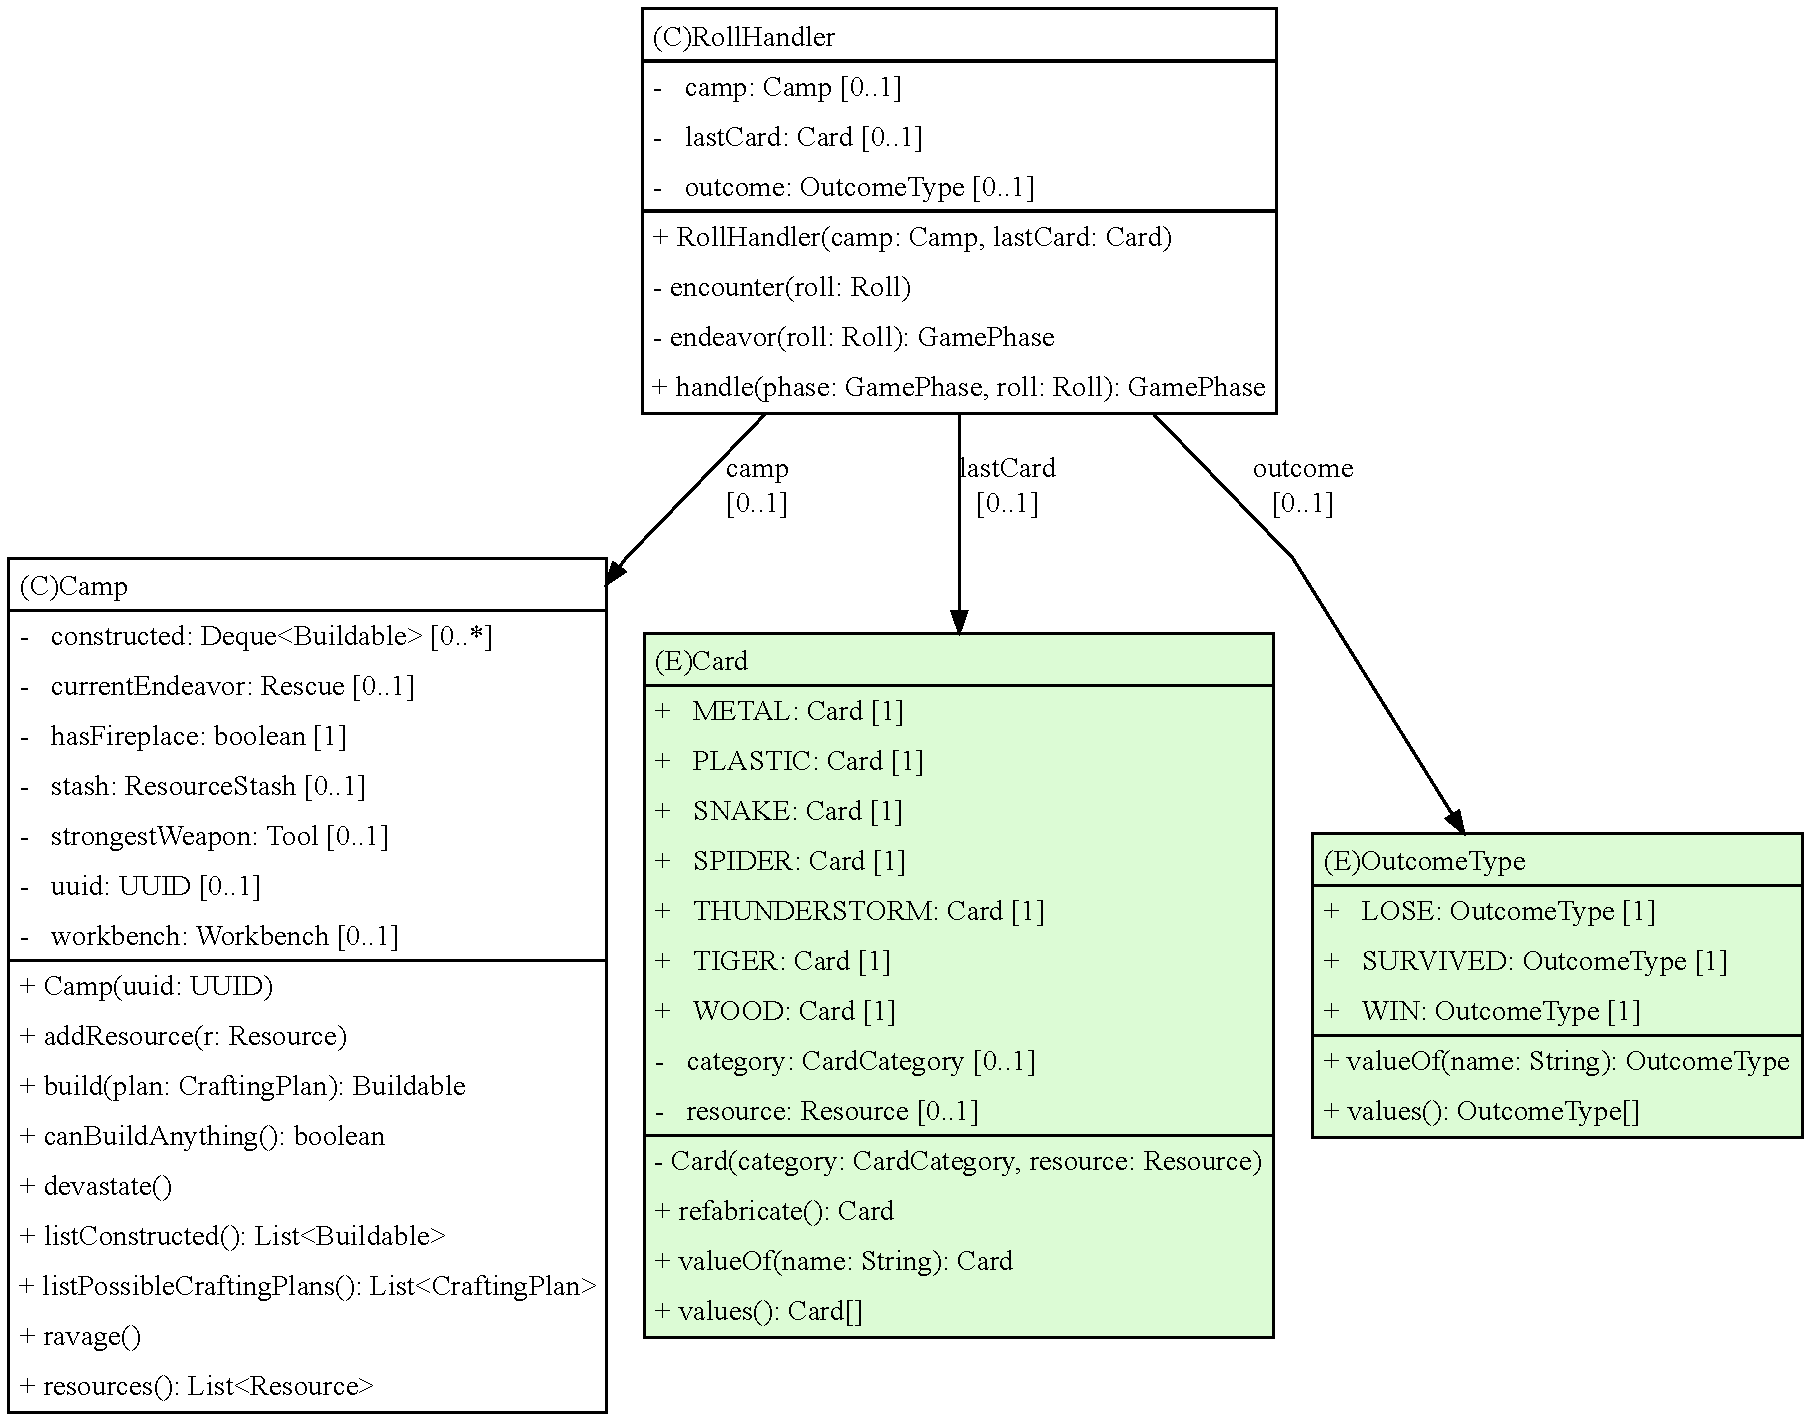
\includegraphics[width=1.\textwidth]{Bilder/RollHandler_structure.pdf} 
	\caption{UML-Diagramm von \textit{application.RollHandler}.}
	\label{fig:srp-RollHandler}
\end{figure} 

\begin{figure}[H]
	\centering
	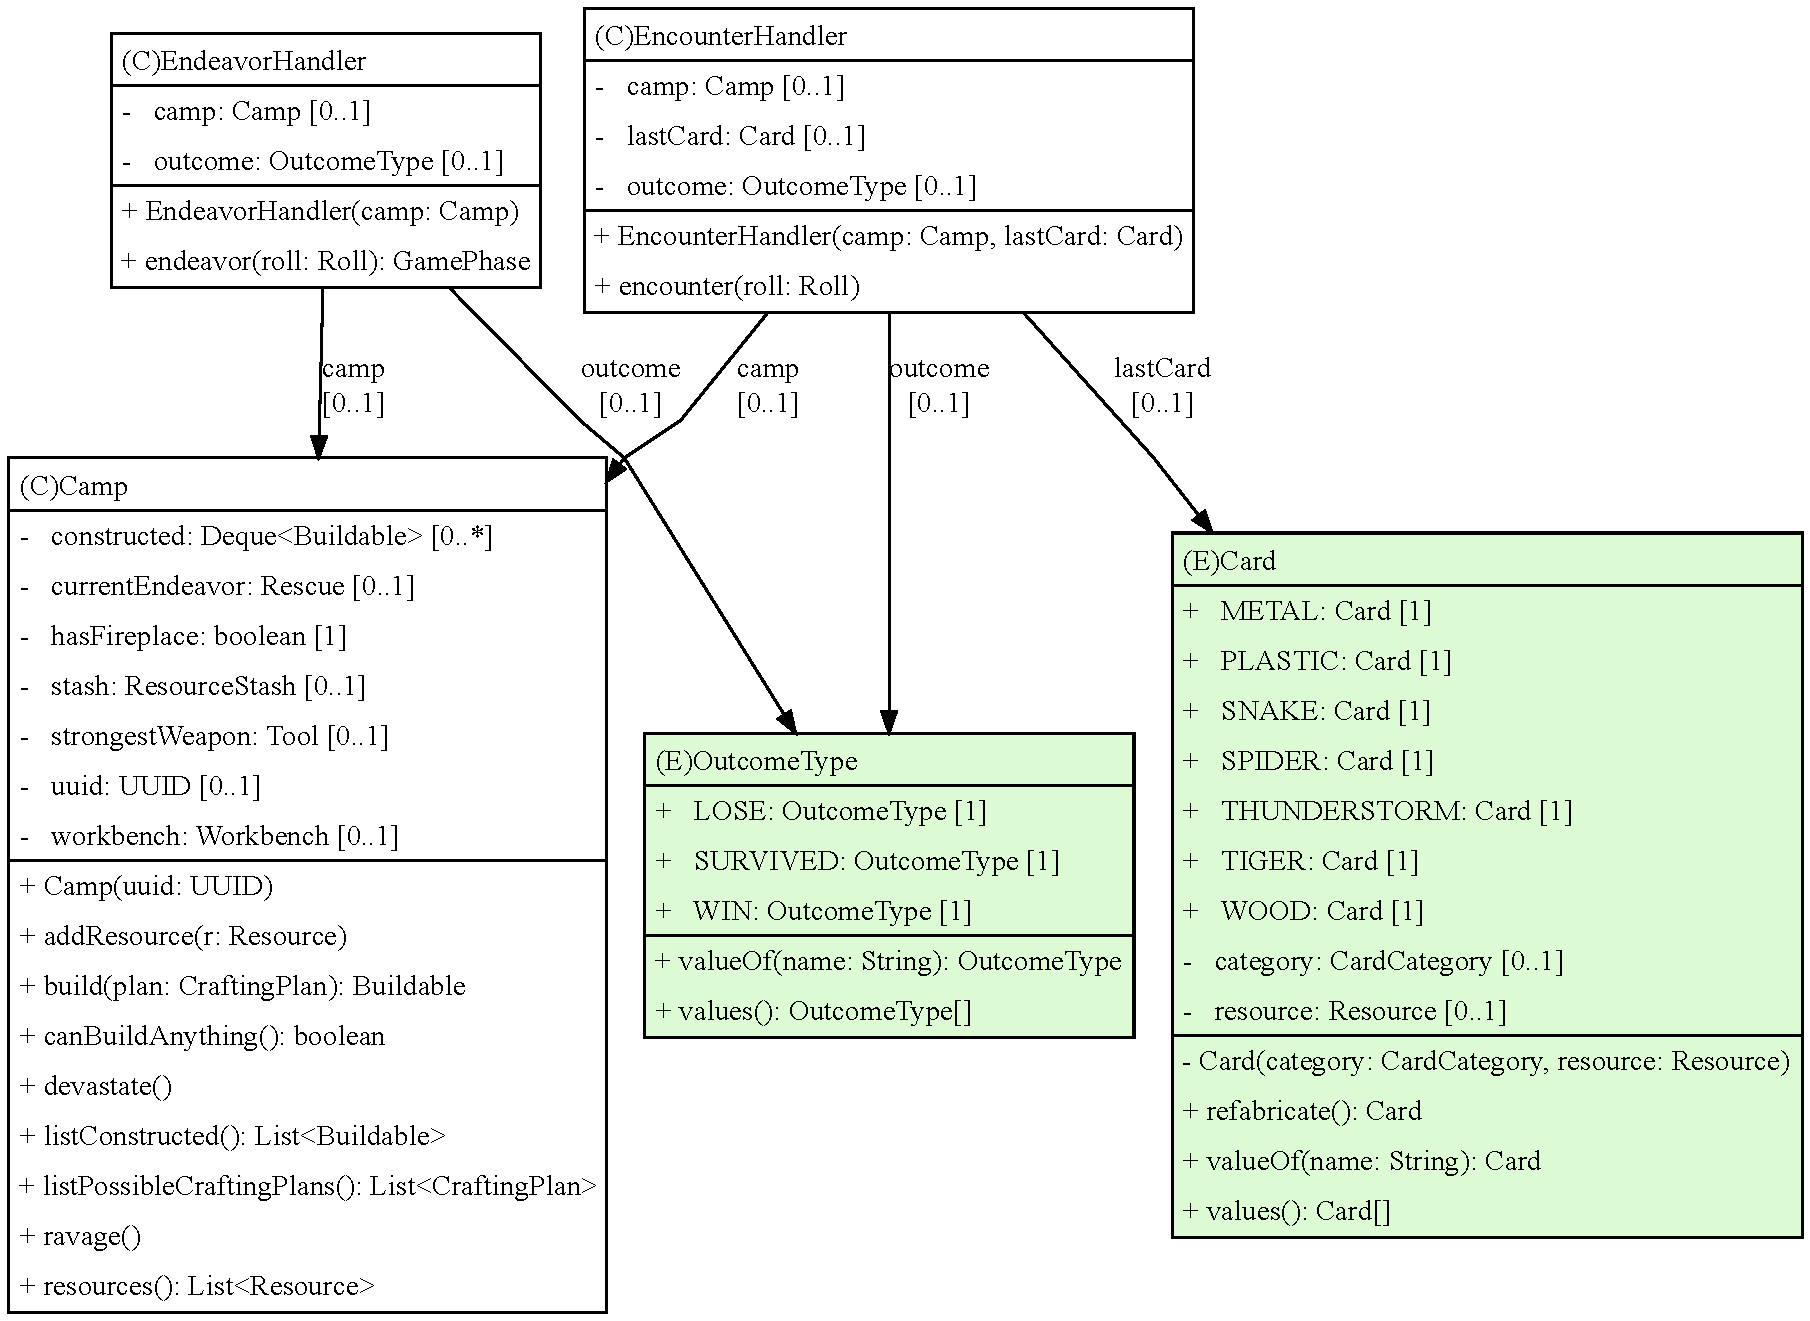
\includegraphics[width=1.\textwidth]{Bilder/RollHandler_fixed_structure.pdf} 
	\caption{\autoref{fig:srp-RollHandler} aufgeteilt in \textit{EndeavorHandler} und \textit{EncounterHandler}.}
	\label{fig:srp-RollHandler-fixed}
\end{figure} 


\section{Analyse Open-Closed-Principle (OCP)}

\subsubsection{Positiv-Beispiel:}

Das Positiv-Beispiel zum OCP wird konstituiert durch das \textit{Command}-Interface aus \texttt{ase.plugin.cli} 
und dessen Implementationen (z.B. \textit{RollDxCommand}) aus \texttt{ase.plugin.cli.commands} wie gezeigt in \autoref{fig:ocp-rolldx}. 
Die Main-Klasse kennt nur das Command-Interface und ruft darauf die \textit{execute}-Methode auf, 
die dann in den unterschiedlichen Command-Implementationen verschiedene Wirkungen auf das übergebene 
\textit{Game} haben. Dies ist auch die Begründung, wieso das OCP hier efüllt wird: Um einen neuen Befehl 
zu implementieren muss lediglich eine weitere Klasse hinzugefügt werden, die das Command-Interface implementiert.
Es muss dazu keine der bestehenden Command-Klassen angepasst oder geändert werden. 

Das OCP ist hier sehr sinnvoll, da für neue Features sehr wahrscheinlich regelmäßig neue Commands hinzugefügt 
werden müssen und dies soll somit möglichst einfach umsetzbar sein und keinen bestehenden Code breaken. 
Zuvor wurden die unterschiedlichen Befehle über zahlreiche \texttt{switch}-Blöcke realisiert 
(siehe z.B. Commit 034a5c28), was Änderungen des Programmcodes an vielen Stellen nötig machte, 
um einen neuen Befehl hinzuzufügen. Außerdem wurden Runtime-Exceptions geworfen, wenn vergessen wurde 
den Code an einer Stelle anzupassen. Durch das neue System müssen \textit{keine} \underline{Änderungen} 
(geschlossen für Änderungen) an vielen Stellen mehr durchgeführt werden, 
sondern nur noch \underline{Additions} durchgeführt werden (offen für Erweiterung).  

\begin{figure}[H]
	\centering
	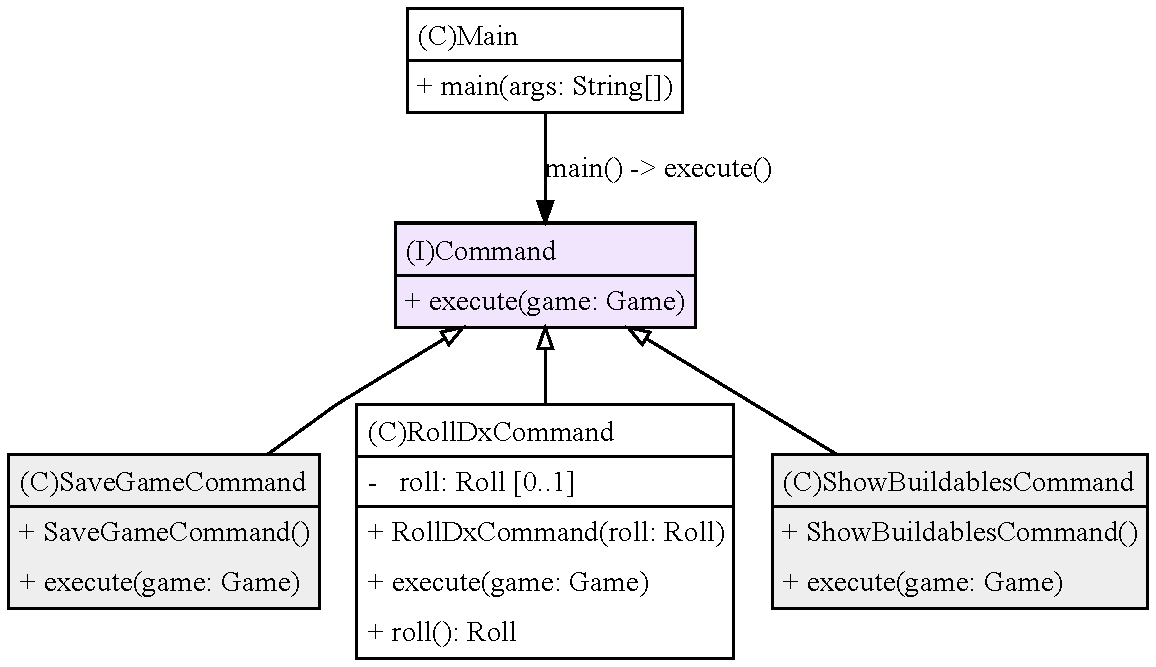
\includegraphics[width=0.7\textwidth]{Bilder/RollDxCommand_structure.pdf} 
	\caption{UML-Klassendiagramm vom \textit{RollDxCommand} und weiteren Commands, 
	wovon die meisten allerdings ausgelassen wurden der Übersichtlichkeit wegen.}
	\label{fig:ocp-rolldx}
\end{figure} 

\subsubsection{Negativ-Beispiel:}


\section{Analyse }

